% ================================================================
%  第 8 章 在数论界面上的相遇 (Encounters at the interface with number theory)
%  依据原书 PDF 第 177--199 页译出；编号审计见文件末尾注释
% ================================================================

\chapter{在数论界面上的相遇}

\epigraph{在调和分析中，我们处理的是作用在复杂函数上的好核；而在数论中，我们得到的是作用在非常光滑函数上的难核.}{Henryk Iwaniec}

\section{来自 Riemann 学位论文的问题}

在他的任教资格论文（Habilitationsschrift）\cite{b194} 中，B.~Riemann 陈述了如下内容: ``[……] 傅里叶级数的用处并不限于物理学中的研究；它们也已成功地应用于纯数学的一个领域，即数论；而且在那里，看来重要的恰恰是考虑那些其三角级数可表示性尚未被研究过的函数.''

Riemann 引入
\begin{align*}
  f(x)=\sum_{n=1}^{\infty}\frac{\{nx\}}{n^{2}},
\end{align*}
并证明 $f$ 恰好在形如 $a/(2b)$（$\gcd(a,2b)=1$）的有理点上不连续，这些点构成实直线的稠密子集.

此外，利用公式
\begin{align*}
  \sum_{n=1}^{\infty}\frac{1}{n^{2}}=\frac{\pi^{2}}{6}\qquad\Bigl(\text{或}\ \sum_{n=0}^{\infty}\frac{1}{(2n+1)^{2}}=\frac{\pi^{2}}{8}\Bigr),
\end{align*}
他证明在这些不连续点处存在跳跃:
\begin{align*}
  f^{-}\Big(\frac{a}{2b}\Big)-f^{+}\Big(\frac{a}{2b}\Big)=\frac{\pi^{2}}{8b^{2}}.
\end{align*}
由于
\begin{align*}
  |f(x)|\leq\frac{\pi^{2}}{6},
\end{align*}
且不连续集是可数的，由此推出 $f$ 是 Riemann 可积的，而其不定积分
\begin{align*}
  F(x)=\int_{0}^{x}f(t)\,\mathrm{d}t
\end{align*}
在那些有理点处是一个连续但不可微的函数:
\begin{align*}
  \lim_{h\to 0^{+}}\frac{F\left(\frac{a}{2b}+h\right)-F\left(\frac{a}{2b}\right)}{h}=f^{+}\Big(\frac{a}{2b}\Big),
\end{align*}
\begin{align*}
  \lim_{h\to 0^{-}}\frac{F\left(\frac{a}{2b}+h\right)-F\left(\frac{a}{2b}\right)}{h}=f^{-}\Big(\frac{a}{2b}\Big).
\end{align*}

在 Riemann 任教资格论文的第 IV 部分，可以找到函数
\begin{align*}
  f(x)=\sum_{n=1}^{\infty}\frac{\{nx\}}{n}.
\end{align*}
我们知道 $f$ 是 Lebesgue 可积的，但不是 Riemann 可积的，因为它的振幅在任何区间上无界.

它可以由三角级数表示:
\begin{align*}
  f(x)=\frac{1}{\pi}\sum_{n=1}^{\infty}\frac{d_{\mathrm{o}}(n)-d_{\mathrm{e}}(n)}{n}\sin(\pi n x),
\end{align*}
其中 $d_{\mathrm{o}}(n)$（相应地，$d_{\mathrm{e}}(n)$）是 $n$ 的奇数（相应地，偶数）因子的个数.

Riemann 写道: ``用形如
\begin{align*}
  \sum_{n=0}^{\infty}C_{n}e^{2\pi i n^{2}x}
\end{align*}
的级数可以得到类似的例子''，当正量 $C_n$ 递减到 $0$、但 $\sum_n C_n = \infty$ 时.

我们在这里遇到一个非常有趣的问题，其解仍是公开的.

\begin{question}\label{ques:8.1}
若 $f$ 是 Lebesgue 可积函数，其傅里叶谱包含于平方数集，是否对每个 $p < 4$ 都有 $\|f\|_p \lesssim \|f\|_1$?
\end{question}

一个等价的表述如下. 设 $S$ 是平方数集示性函数给出的傅里叶乘子算子，即若 $f$ 有傅里叶级数 $\sum \widehat{f}(k)e^{2\pi ikx}$，则 $Sf$ 的傅里叶级数由
\begin{align*}
  \sum_{n=0}^{\infty}\widehat{f}(n^{2})e^{2\pi i n^{2}x}
\end{align*}
给出.

\begin{question}\label{ques:8.2}
$S$ 是否是从 $L^2[0,1]$ 到 $L^p[0,1]$（$2 \leq p < 4$）的有界算子?
\end{question}

由对偶，它等价于 $S$ 对每个 $q > 4/3$ 从 $L^q[0,1]$ 到 $L^2[0,1]$ 的有界性. 肯定的回答会有非常有趣的算术推论. 例如，它将蕴含: 长度为 $N$ 的任何等差数列 $\{a + br : 0 \leq r \leq N - 1\}$ 对每个 $\varepsilon > 0$ 至多含有 $O(N^{1/2+\varepsilon})$ 个平方数（关于这一问题的更多细节见文献 \cite{b180}）.

若 $G(x) = \sum_{r=0}^{N-1} e^{2\pi i(a+br)x}$，则对 $p > 1$ 有 $\|G\|_p \sim N^{(p-1)/p}$. 另一方面，若 $n_1^2 < n_2^2 < \cdots < n_k^2$ 是等差数列 $\{a+br\}_{r=0,\ldots,N-1}$ 所含的平方数，并假设我们关于 $S$ 的问题有肯定回答，则得到
\begin{align*}
  k^{1/2}=\|S(G)\|_{2}\lesssim\|S(G)\|_{p}\lesssim N^{(p-1)/p}
\end{align*}
对每个 $p > 4/3$ 成立，由此得 $k = O(N^{1/2+\varepsilon})$，其中 $p = 1/(3/4 - \varepsilon)$.

给定 $a \in \Z$ 与 $r \in \Z^+$，定义
\begin{align*}
  \sigma(N;a,r)=\#\{m^{2}=a+nr;\ 0\leq r<N\},\qquad
  \sigma(N)=\sup_{a,r}\sigma(N;a,r).
\end{align*}
有一个归功于 P.~Erdős 的猜想:
\begin{align*}
  \sigma(N)=O(N^{1/2+\varepsilon}),\qquad \text{对所有 } \varepsilon>0.
\end{align*}
不难看出 $G(N) = O(N^{1/2})$ 并不成立；上面的推理表明，关于乘子 $S$ 的问题的肯定回答蕴含 Erdős 猜想. 然而，目前已知的最好结果是 $\sigma(N) = O(N^{3/5+\varepsilon})$（对所有 $\varepsilon > 0$）. 这归功于 Bombieri--Zannier \cite{b174}.

\section{平方数的 $B_{2}[\infty]$-序列}

用 $r(n)$ 表示整数 $n$ 表为两平方和的表法个数. 它是一个杰出的算术函数，其研究是数论中熟悉的课题. 这个函数有相当``不规则''的行为，因为值 $r(n)$ 依赖于 $n$ 的素因子分解.

另一方面，众所周知它的平均值满足
\begin{align*}
  \sum_{n\leq x}r(n)\sim\pi x,\qquad x\to\infty.
\end{align*}
这种``不规则性''的一个特别有趣的表达是: $\sum_{n \leq x} r^2(n)$ 的量级严格大于 $\sum_{n \leq x} r(n)$. 更精确地,
\begin{align*}
  \frac{\sum_{n\leq x}r^{2}(n)}{\sum_{n\leq x}r(n)}\gtrsim\log x.
\end{align*}
于是自然考虑下面这一类的序列.

\begin{definition}\label{def:8.3}
称正整数序列 $\{n_k\}$ 具有性质 $B_2[\infty]$，或者说它是 $B_2[\infty]$-序列，若
\begin{align*}
  \limsup_{x\to\infty}\frac{\sum_{n\leq x}r^{2}(n)}{\sum_{n\leq x}r(n)}<+\infty,
\end{align*}
其中 $r(n) = \#\{n = n_k + n_j,\ n_k \leq n_j\}$.
\end{definition}

这个定义也是 $B_2[g]$-序列概念的自然推广，后者是指对每个 $n$ 有 $r(n) \leq g$ 的序列. 细节与应用参见 \cite{b189}.

正如我们已经指出的，整个平方数序列不是 $B_2[\infty]$-序列. 似乎是 J.~E.~Littlewood 首先观察到这一事实在具有与平方数相似增长的序列中是``非典型的''. 在他的博士论文中，A.~O.~L.~Atkin（见 \cite{b171}）证实了 Littlewood 的预言，证明了与平方数非常接近的 $B_2[\infty]$-序列的存在性（$n_k = k^2 + O(\log k)$）. 他还观察到，满足 $n_k = k^2 + O(\sqrt{\log k})$ 的任何序列 $\{n_k\}$ 都不具有性质 $B_2[\infty]$.

后来，P.~Erdős 与 A.~Rényi \cite{b185} 用概率方法证明了: 在某种意义下，与平方数接近的几乎每个序列（$n_k = k^2(1 + o(1))$）都是 $B_2[\infty]$ 的. 在 \cite{b171} 与 \cite{b185} 中，所考虑的序列都保持平方数的增长，但其项不是平方数. 下面我们将向相反方向进行，构造具有所需性质 $B_2[\infty]$、且增长速度适度的平方数子序列.

\begin{theorem}\label{thm:8.4}
存在无穷平方数序列 $a_1^2 < a_2^2 < \cdots < a_k^2 < \cdots$，满足性质 $B_2[\infty]$，且 $a_k^2 \lesssim k^2\log^2 k$.
\end{theorem}

\begin{proof}
我们将显式地构造一族这样的序列. 设
\begin{align*}
  I_{j}^{\nu}=\left\{2n\ \Big|\ 2^{j}(1+\nu/j)\leq 2n<2^{j}(1+(\nu+1)/j)\right\},\qquad j=1,\ldots,\ 0\leq\nu\leq j-1.
\end{align*}
对每个 $j$ 选取 $v_{j}$ 后，考虑集合
\begin{align*}
  I^{(\nu)}=\bigcup_{j}I_{j}^{\nu_{j}},\qquad
  A^{(\nu)}=\{a_{k}^{2}\mid a_{k}\in I^{(\nu)}\}.
\end{align*}
我们断言 $A^{(\nu)}$ 满足定理 8.4 要求的条件. （为简化记号，我们考虑 $\nu_j = 0$ 的情形；对一般值 $\nu_j$，$j = 1, 2, \ldots$，证明相同.）

显然有
\begin{align*}
  a_{[2^{j-1}/j]}\leq 2^{j}+2^{j}/j\leq 2^{j+1},
\end{align*}
因此，给定 $k$，存在 $j$，使 $2^{j-1}/j \leq k < 2^j/(j+1)$. 则
\begin{align*}
  a_{k}\leq a_{[2^{j}/(j+1)]}<2^{j+2}\lesssim k\log k.
\end{align*}
考虑
\begin{align*}
  r(n)=\#\{n=a_{k}^{2}+a_{l}^{2}\mid a_{k}\leq a_{l}\ \text{且 } a_{k},a_{l}\in I=\bigcup_{j}I_{j}^{0}\}.
\end{align*}
有下列不等式:
\begin{equation}\label{eq:8.1}
  \sum_{n\leq x}r(n)=\sum_{\substack{a_{k}^{2}+a_{l}^{2}\leq x\\ a_{k}\leq a_{l}}}1
  \geq\frac{1}{2}\Big(\sum_{a_{k}^{2}\leq x/2}1\Big)^{2}
  \gtrsim\frac{x}{\log^{2}x}.
\end{equation}
因此，为证明定理，只须证明下面的估计:
\begin{align*}
  \sum_{n\leq x}r^{2}(n)\lesssim\frac{x}{\log^{2}x}.
\end{align*}
为看出这一点，对每个 $j$ 定义函数
\begin{align*}
  r_{j}(n)=\#\{n=a_{k}^{2}+a_{l}^{2}\mid a_{k}\leq a_{l}\ \text{且 } a_{k},a_{l}\in I_{j}^{0}\}.
\end{align*}
则
\begin{align*}
  \sum_{n\leq x}r^{2}(n)\lesssim\Big[\sum_{j\leq[\log_{4}x]}\Big(\sum_{n}r_{j}^{2}(n)\Big)^{1/2}\Big]^{2}.
\end{align*}
这是傅里叶级数 Littlewood--Paley 理论，连同把和 $\sum_{n \leq x} r^2(n)$ 自然地解释为相应三角多项式的 $L^4$-范数的推论:
\begin{align*}
  \sum_{n\leq x}r^{2}(n)
  &\simeq\Big\|\sum_{j\leq(\log_{2}x)/2}\sum_{n\in I^{0}_{j}}e^{2\pi i n^{2}x}\Big\|_{4}^{4}
  \simeq\Big\|\Big(\sum_{j\leq(\log_{2}x)/2}\Big|\sum_{n\in I^{0}_{j}}e^{2\pi i n^{2}x}\Big|^{2}\Big)^{1/2}\Big\|_{4}^{4}\\
  &\lesssim\Big(\sum_{j\leq(\log_{2}x)/2}\Big\|\sum_{n\in I^{0}_{j}}e^{2\pi i n^{2}x}\Big\|_{4}^{2}\Big)^{2}
  \simeq\Big(\sum_{j\leq(\log_{2}x)/2}\Big(\sum_{n}r^{2}_{j}(n)\Big)^{1/2}\Big)^{2}.
\end{align*}
我们使用标准记号（见记号一节）$A(z) \simeq B(z)$，若存在常数 $0 < C_1 \leq C_2 < \infty$，使对每个 $z$ 有 $C_1A(z) \leq B(z) \leq C_2A(z)$.

我们断言
\begin{equation}\label{eq:8.2}
  \sum_{n}r_{j}^{2}(n)\lesssim\left(\frac{2^{j}}{j}\right)^{2}.
\end{equation}
于是得到
\begin{align*}
  \sum_{n\leq x}r^{2}(n)\lesssim\Big(\sum_{j\leq(\log_{2}x)/2}\frac{2^{j}}{j}\Big)^{2}
  \lesssim\frac{x}{\log^{2}x}.
\end{align*}
为完成证明，必须证明估计 \eqref{eq:8.2}. 分两步: 先陈述一个引理.

\begin{lemma}\label{lem:8.5}
若 $r_j(n) \geq 2$，则 $r_j^2(n) \lesssim F(n)$，其中 $F(n)$ 是下列不等式组的整数解 $(a_1, b_1, a_2, b_2)$ 的个数:
\begin{align*}
  0<\left|\frac{a_{1}}{b_{1}}\right|<\frac{1}{j},\qquad
  0<\left|\frac{a_{2}}{b_{2}}-1\right|<\frac{1}{j},\qquad
  n=(a_{1}^{2}+b_{1}^{2})\cdot(a_{2}^{2}+b_{2}^{2}).
\end{align*}
\end{lemma}

假设该引理成立，可以完成 \eqref{eq:8.2} 的证明. 固定 $j$，有
\begin{align*}
  \sum_{n}r_{j}^{2}(n)\leq\sum_{r_{j}(n)=1}r_{j}(n)+\sum_{r_{j}(n)\geq 2}r_{j}^{2}(n).
\end{align*}
显然第一项满足估计 $\sum r_j(n) \lesssim (2^j/j)^2$.

由引理 8.5，第二项以
\begin{align*}
  2\left(2^{j}\right)^{2}\leq\left(a_{1}^{2}+b_{1}^{2}\right)\left(a_{2}^{2}+b_{2}^{2}\right)
  \leq 2\left(2^{j}+2^{j}/j\right)^{2},\qquad
  0<\left|\frac{a_{1}}{b_{1}}\right|<1/j,\qquad
  0<\left|\frac{a_{2}}{b_{2}}-1\right|<\frac{1}{j}
\end{align*}
的解 $(a_{1}, b_{1}, a_{2}, b_{2})$ 的个数为界. 固定 $a_{1}$ 与 $b_{1}$，估计满足
\begin{align*}
  \sqrt{2}\frac{2^{j}}{\sqrt{a_{1}^{2}+b_{1}^{2}}}\leq\sqrt{a_{2}^{2}+b_{2}^{2}}
  \leq\frac{\sqrt{2}\left(2^{j}+2^{j}/j\right)}{\sqrt{a_{1}^{2}+b_{1}^{2}}},\qquad
  0<\left|\frac{a_{2}}{b_{2}}-1\right|<\frac{1}{j}
\end{align*}
的点对 $(a_{2}, b_{2})$ 的个数. 可以把每个解 $(a_{2}, b_{2})$ 与图中所述区域内的一个格点等同起来.

\begin{center}
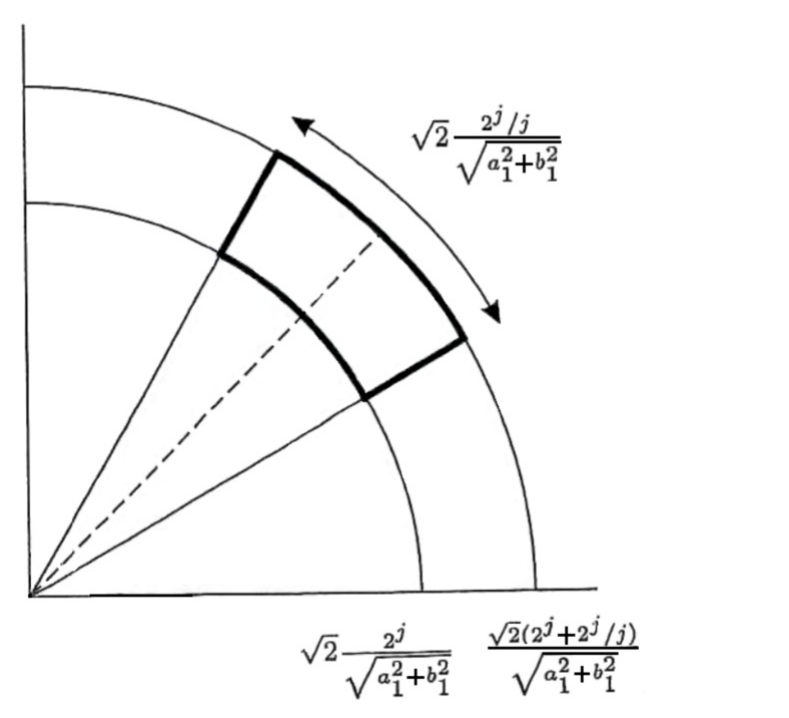
\includegraphics[width=0.36\textwidth]{figs/fig-8-riemann.png}
\end{center}

条件 $0 < |a_2/b_2 - 1| < 1/j$ 给出 $b_2 > j$，因此,
\begin{align*}
  \sqrt{2}\frac{2^{j}/j}{\sqrt{a_{1}^{2}+b_{1}^{2}}}\gtrsim 1,
\end{align*}
这使得该区域内的格点数可以用它的面积来估计. 于是
\begin{align*}
  \sum_{r_{j}(n)\geq 2}r_{j}^{2}(n)
  \lesssim\sum_{\substack{a_{1},b_{1}\\ 0<|a_{1}/b_{1}|<1/j}}\frac{4^{j}}{(a_{1}^{2}+b_{1}^{2})j^{2}}
  \lesssim\sum_{b_{1}<2^{j}}\frac{4^{j}}{b_{1}j^{3}}
  \lesssim\frac{4^{j}}{j^{2}},
\end{align*}
由此容易得出不等式 \eqref{eq:8.2}.
\end{proof}

\begin{proof}[引理~\ref{lem:8.5} 的证明]
首先观察（细节见 \cite{b24}）: 若 $n \equiv 0 \pmod 4$ 表为两平方和有两种不同的分解 $n = a^2 + b^2 = c^{2}+d^{2}$，则存在整数 $a_{1}, b_{1}, a_{2}$ 与 $b_{2}$，使
\begin{align*}
  n=\left(a_{1}^{2}+b_{1}^{2}\right)(a_{2}^{2}+b_{2}^{2}),
\end{align*}
\begin{align*}
  \frac{a_{1}}{b_{1}}=\tan\Big(\frac{\arctan(a/b)+\arctan(c/d)}{2}\Big),\qquad
  \frac{a_{2}}{b_{2}}=\tan\Big(\frac{\arctan(a/b)-\arctan(c/d)}{2}\Big).
\end{align*}
设 $n = a_r^2 + b_r^2 = a_s^2 + b_s^2$ 是 $n$ 表为两平方和的两种不同表示，满足
\begin{align*}
  2^{j}\leq a_{r}\leq b_{r}\leq 2^{j}+\frac{2^{j}}{j},\qquad
  2^{j}\leq a_{s}\leq b_{s}\leq 2^{j}+\frac{2^{j}}{j},
\end{align*}
\begin{align*}
  a_{r}\equiv b_{r}\equiv a_{s}\equiv b_{s}\equiv 0\pmod{2}.
\end{align*}
由前面的论证，存在 $a_{1}, b_{1}, a_{2}$ 与 $b_{2}$，使
\begin{align*}
  n=\left(a_{1}^{2}+b_{1}^{2}\right)(a_{2}^{2}+b_{2}^{2}),
\end{align*}
\begin{align*}
  \frac{a_{1}}{b_{1}}=\tan\Big(\frac{\arctan(a_{r}/b_{r})+\arctan(a_{s}/b_{s})}{2}\Big),
\end{align*}
\begin{align*}
  \frac{a_{2}}{b_{2}}=\tan\Big(\frac{\arctan(a_{r}/b_{r})-\arctan(a_{s}/b_{s})}{2}\Big).
\end{align*}
对 $a_{r}$，$b_{r}$，$a_{s}$ 与 $b_{s}$ 所加的条件容易给出
\begin{align*}
  \left|\frac{a_{2}}{b_{2}}\right|<\frac{1}{j},\qquad
  \left|\frac{a_{1}}{b_{1}}-1\right|<\frac{1}{j}.
\end{align*}
另一方面，两个量都严格大于 $0$，因为否则我们不可能从 $n$ 表为两平方和的两种不同表示出发.

每对不同表示
\begin{align*}
  \{n=a_{r}^{2}+b_{r}^{2}=a_{s}^{2}+b_{s}^{2},\ a_{s}\equiv b_{s}\equiv a_{r}\equiv b_{r}\equiv 0 \pmod 2\}
\end{align*}
产生不同的角，从而产生不同的整数 $a_1, b_1, a_2$ 与 $b_2$. 因此 $\binom{r_j(n)}{2}$ 以问题
\begin{align*}
  n=\left(a_{1}^{2}+b_{1}^{2}\right)\left(a_{2}^{2}+b_{2}^{2}\right),\qquad
  0<\left|\frac{a_{1}}{b_{1}}\right|<\frac{1}{j},\qquad
  0<\left|\frac{a_{2}}{b_{2}}-1\right|<\frac{1}{j}
\end{align*}
的解数为上界. 引理由观察 $r_j(n) \geq 2$ 时 $r_j^2(n) \leq 4\binom{r_j(n)}{2}$ 得出.
\end{proof}

\begin{remark}\label{rem:8.6}
不难看出，满足 $n_k^2 = o(k^2\log k)$ 的平方数子序列 $\{n_k^2\}$ 不可能具有性质 $B_2[\infty]$.

此外，可以构造增长非常快、却仍然不是 $B_2[\infty]$-序列的平方数序列.
\end{remark}

\section{平方频率的傅里叶级数}

关于频率为平方数的傅里叶级数的 $L^{p}$-特征的问题，在系数的单调性条件下有令人满意的答案.

\begin{proposition}\label{prop:8.7}
假设 $\{a_n\}$ 是非负实数的单调递减序列，且 $\sum_{n=0}^{\infty} a_n e^{2\pi i n^2x}$ 是可积函数 $f$ 的傅里叶级数. 则对每个 $p$，$1 \leq p < 4$，有 $f \in L^p[0,1]$，并满足估计
\begin{align*}
  \|f\|_{p}\lesssim\|f\|_{1}.
\end{align*}
\end{proposition}

上述命题的证明将基于下面的事实.

\begin{lemma}\label{lem:8.8}
设 $f$ 在 $[0, 1]$ 上连续，且满足
\begin{enumerate}
\item[(i)] $\|f\|_{\infty} \leq N$，$\|f\|_2 \leq N^{1/2}$；
\item[(ii)] 若 $|x - p/q| \leq 1/q^2$，则
\begin{align*}
  |f(x)|\leq C_{0}\left\{q^{1/k}+\frac{N}{q^{1/k}}\right\},\qquad \text{对某个常数 } C_{0}.
\end{align*}
\end{enumerate}
则 $f$ 满足 $2k$-弱型不等式
\begin{align*}
  \mu\{x:|f(x)|>\alpha>0\}\leq C\frac{N^{k}}{\alpha^{2k}}
\end{align*}
对每个 $\alpha > 0$ 成立，其中常数 $C = C(C_0)$ 与 $\alpha$ 和 $N$ 无关，$\mu$ 表示 $[0,1]$ 中的 Lebesgue 测度.
\end{lemma}

\begin{proof}
不失一般性，可以假设 $C_0 = 1$，因为若 $C_0 > 1$，只需考虑函数 $f/C_0$. 证明将等价于: 对每个 $\alpha > 0$,
\begin{align*}
  \mu(E_{\alpha})=\mu\{|f(x)|\geq 2N^{1/2}\alpha\}\leq\widetilde{C}\frac{1}{\alpha^{2k}},
\end{align*}
其中 $\widetilde{C}$ 与 $N$ 和 $\alpha$ 无关. 注意只须在 $\frac{1}{2}N^{1/2} \geq \alpha \geq 1$ 时证明，因为 $\alpha < 1$ 时不等式平凡化，而 $\alpha \geq \frac{1}{2}N^{1/2}$ 时 $E_{\alpha} = \emptyset$. 若
\begin{align*}
  x=\frac{1}{x_{1}+\frac{1}{x_{2}+\frac{1}{x_{3}+\cdots}}}
\end{align*}
是无理数 $x \in E_\alpha$ 的连分数展开，渐近分数为 $\{P_\nu/Q_\nu\}$，则下列成立:
\begin{align*}
  Q_{\nu}^{1/k}+\frac{N}{Q_{\nu}^{1/k}}\geq 2N^{1/2}\alpha.
\end{align*}
即，对每个 $\nu$,
\begin{align*}
  \text{或}\quad Q_{\nu}^{1/k}\geq N^{1/2}\alpha,\qquad
  \text{或}\quad N/Q_{\nu}^{1/k}\geq N^{1/2}\alpha.
\end{align*}
有两种可能的情形:

情形 1. $Q_1^{1/k} \geq N^{1/2}\alpha$，即 $Q_1 \geq N^{k/2}\alpha^k$.

由于 $x \leq 1/Q_1$，有 $x \in I_0 = [0, \frac{1}{N^{k/2}\alpha^k}]$，且
\begin{align*}
  \mu(I_{0})=\frac{1}{N^{k/2}\alpha^{k}}\leq\frac{1}{2^{k}\alpha^{2k}}.
\end{align*}

情形 2. 存在 $\nu \geq 1$，使
\begin{align*}
  \frac{N}{Q_{\nu}^{1/k}}\geq N^{1/2}\alpha,\qquad \text{即}\quad Q_{\nu}\leq\frac{N^{k/2}}{\alpha^{k}},
\end{align*}
以及
\begin{align*}
  Q_{\nu+1}^{1/k}\geq N^{1/2}\alpha,\qquad \text{即}\quad Q_{\nu+1}\geq N^{k/2}\alpha^{k}.
\end{align*}
有
\begin{align*}
  \left|x-\frac{P_{\nu}}{Q_{\nu}}\right|\leq\frac{1}{Q_{\nu}Q_{\nu+1}}
  \leq\frac{1}{Q_{\nu}}\frac{1}{N^{k/2}\alpha^{k}},
\end{align*}
即
\begin{align*}
  x\in\Bigl(\frac{P_{\nu}}{Q_{\nu}}-\frac{1}{Q_{\nu}}\frac{1}{N^{k/2}\alpha^{k}},
  \frac{P_{\nu}}{Q_{\nu}}+\frac{1}{Q_{\nu}}\frac{1}{N^{k/2}\alpha^{k}}\Bigr).
\end{align*}
给定满足 $r < s$，$\gcd(r, s) = 1$，$s \leq N^{k/2}/\alpha^k$ 的整数 $r$ 与 $s$，考虑区间
\begin{align*}
  I_{r,s}=\Bigl(\frac{r}{s}-\frac{1}{s}\frac{1}{N^{k/2}\alpha^{k}},
  \frac{r}{s}+\frac{1}{s}\frac{1}{N^{k/2}\alpha^{k}}\Bigr).
\end{align*}
则前面的观察给出包含关系
\begin{align*}
  E_{\alpha}\setminus\{\text{有理数}\}\subset I_{0}\bigcup\Big(\bigcup_{r,s}I_{r,s}\Big).
\end{align*}
因此,
\begin{align*}
  \mu(E_{\alpha})
  &\leq\mu(I_{0})+\sum_{\substack{r=1\\ (r,s)=1}}^{s-1}\sum_{s=1}^{N^{k/2}/\alpha^{k}}\mu(I_{r,s})
  \leq\frac{1}{\alpha^{2k}}+\sum_{s=1}^{N^{k/2}/\alpha^{k}}\sum_{r=1}^{s-1}
   \frac{2}{s}\frac{1}{N^{k/2}\alpha^{k}}\\
  &\leq\frac{1}{\alpha^{2k}}+\sum_{s=1}^{N^{k/2}/\alpha^{k}}\frac{2}{N^{k/2}\alpha^{k}}
  \leq\frac{3}{\alpha^{2k}}.
\end{align*}
\end{proof}

接下来考虑三角多项式
\begin{align*}
  S_{N}(x;y)=\sum_{n=1}^{N}e^{2\pi i(n^{2}x+ny)}
\end{align*}
及其 Carleson 极大函数
\begin{align*}
  C_{N}^{*}(x;y)=\sup_{1\leq M\leq N}|S_{M}(x;y)|.
\end{align*}
现在用 Carleson 极大定理继续命题 8.7 的证明，证明对每个 $y \in [0,1]$，$S_N(x; y)$ 在 $k = 2$ 的情形满足引理 8.8 的假设.

\begin{lemma}\label{lem:8.9}
设 $x$ 有形如 $|x - p/q| \leq 1/q^2$ 的有理逼近，$1 \leq q \leq N^2$，$\gcd(p, q) = 1$. 则
\begin{align*}
  C_{N}^{*}(x;y)\lesssim\left\{q^{1/2}+\frac{N}{q^{1/2}}\right\}.
\end{align*}
\end{lemma}

这个结果 Hardy 与 Littlewood \cite{b187,b188} 已知，他们用 $\theta$-函数的近似函数方程证明了它. 下面 E.~Bombieri 的证明，见 \cite{b173}，通过使用 Carleson 定理 \cite{b175} 强调了数论与调和分析之间的联系.

\begin{proof}
首先注意，若 $|x - x_0| \leq \frac{1}{4N^2}$ 且 $|y - y_0| \leq \frac{1}{4N}$，则有不等式
\begin{align*}
  C_{N}^{*}(x;y)\leq 100C_{N}^{*}(x_{0};y_{0}).
\end{align*}
这是因为
\begin{align*}
  S_{M}(x;y)
  &=\sum_{n=1}^{M}e^{2\pi i(n^{2}x+ny)}
  =\sum_{n=1}^{M}e^{2\pi i(n^{2}x_{0}+ny_{0})}\cdot e^{2\pi i(n^{2}(x-x_{0})+n(y-y_{0}))}\\
  &=\sum_{n=1}^{M}\left(S_{n}(x_{0};y_{0})-S_{n-1}(x_{0};y_{0})\right)e^{2\pi i(n^{2}(x-x_{0})+n(y-y_{0}))}\\
  &=\sum_{n=1}^{M-1}S_{n}(x_{0};y_{0})\left(e^{2\pi i(n^{2}(x-x_{0})+n(y-y_{0}))}
   -e^{2\pi i((n+1)^{2}(x-x_{0})+(n+1)(y-y_{0}))}\right)\\
  &\quad+S_{M}(x_{0};y_{0})e^{2\pi i(M^{2}(x-x_{0})+M(y-y_{0}))}.
\end{align*}
对 $M$，$1 \leq M \leq N$，取上确界，得
\begin{align*}
  C_{N}^{*}(x;y)
  &\leq 2C_{N}^{*}(x_{0};y_{0})\left[1+\sum_{n=1}^{N}(|x-x_{0}|4\pi n+4\pi|y-y_{0}|)\right]\\
  &\leq 100C_{N}^{*}(x_{0};y_{0}).
\end{align*}
其次，对所有 $M$，$1 \leq M \leq N$，有下列不等式:
\begin{align*}
  C_{N}^{*}(x;y)\leq 2C_{2N}^{*}(x;y-2Mx),
\end{align*}
因为对所有 $K \leq N$,
\begin{align*}
  \left|S_{K}(x;y)\right|
  &=\Big|\sum_{n=1}^{K}e^{2\pi i(n^{2}x+ny)}\Big|
  =\Big|\sum_{n=M+1}^{K+M}e^{2\pi i((n-M)^{2}x+(n-M)y)}\Big|\\
  &=\Big|\sum_{n=M+1}^{K+M}e^{2\pi i(n^{2}x+n(y-2Mx))}\Big|
  \leq 2C_{2N}^{*}(x;y-2Mx).
\end{align*}
把不等式平方并对 $M$ 取平均，得
\begin{align*}
  |C_{N}^{*}(x;y)|^{2}
  &\leq\frac{4}{N}\sum_{M=1}^{N}|C_{2N}^{*}(x;y-2Mx)|^{2}\\
  &\leq\frac{4}{N}\sum_{n=1}^{M}(100)^{2}8N\int_{I(2Mx-y)}|C_{2N}^{*}(x;y_{0})|^{2}\,\mathrm{d}y_{0},
\end{align*}
其中 $I(z) = \{w : |z - w| \leq \frac{1}{8N}\}$. 初等计算给出区间族 $\{I_{(2M x - y)}\}$ 重叠的上界:
\begin{align*}
  \Big\|\sum_{M=1}^{N}\chi_{I_{(2M x-y)}}\Big\|_{\infty}\lesssim\Big(\frac{N}{q}+\frac{q}{N}\Big),
\end{align*}
应用 Carleson 极大定理，得
\begin{align*}
  C_{N}^{*}(x;y)^{2}\lesssim\left\{q+\frac{N^{2}}{q}\right\}.
\end{align*}
\end{proof}

\begin{proof}[命题~\ref{prop:8.7} 的证明]
考虑极大函数
\begin{align*}
  C_{N}^{*}(x)=\sup_{1\leq M\leq N}\Big|\sum_{n=1}^{M}e^{2\pi i n^{2}x}\Big|.
\end{align*}
则引理 8.8 与 8.9 给出估计
\begin{align*}
  \mu(\{C_{N}^{*}(x)\geq 2N^{1/2}\alpha\})\lesssim\frac{1}{\alpha^{4}},
\end{align*}
特别地，得到
\begin{align*}
  \|C_{N}^{*}\|_{p}\leq C_{p}N^{1/2},\qquad 2\leq p<4.
\end{align*}
给定傅里叶级数 $f = \sum a_n e^{2\pi i n^2 x}$，有 Littlewood--Paley 范数等价
\begin{align*}
  \|f\|_{p}\simeq\Big\|\Big(\sum_{k}|\Delta_{k}(x)|^{2}\Big)^{1/2}\Big\|_{p},\qquad 1<p<\infty,
\end{align*}
其中
\begin{align*}
  \Delta_{k}(x)=\sum_{n=2^{k}}^{2^{k+1}-1}a_{n} e^{2\pi i n^{2}x}.
\end{align*}
特别地，对 $2 \leq p < 4$ 有
\begin{align*}
  \|f\|_{p}
  &\lesssim\Big[\int_{0}^{1}\Big(\sum_{k}|\Delta_{k}(x)|^{2}\Big)^{p/2}\Big]^{\frac{2}{p}\cdot\frac{1}{2}}
  \leq\Big[\sum_{k}\Big(\int_{0}^{1}|\Delta_{k}|^{p}\Big)^{2/p}\Big]^{1/2}\\
  &=\Big(\sum_{k}\|\Delta_{k}\|_{p}^{2}\Big)^{1/2}.
\end{align*}
但
\begin{align*}
  \Delta_{k}(x)
  &=\sum_{n=2^{k}}^{2^{k+1}-1}a_{n} e^{2\pi i n^{2}x}
  =\sum_{n=2^{k}}^{2^{k+1}-1}a_{n}\left[S_{n}(x)-S_{n-1}(x)\right]\\
  &=\sum_{n=2^{k}}^{2^{k+1}-1}(a_{n}-a_{n+1})S_{n}(x)+a_{2^{k+1}-1}S_{2^{k+1}-1}(x),
\end{align*}
其中 $S_{n}(x)$ 表示 $f$ 的部分和. 由于系数单调递减，得
\begin{align*}
  \left|\Delta_{k}(x)\right|\leq 2C_{2^{k+1}}^{*}(x)\cdot a_{2^{k}}.
\end{align*}
因此,
\begin{align*}
  \|f\|_{p}\lesssim\Big(\sum_{k}a_{2^{k}}^{2}\cdot 2^{k}\Big)^{1/2}\lesssim\|f\|_{2}.
\end{align*}
\end{proof}

\section{Riemann 图象的分形维数}

在他的学位论文中，Riemann 还引入了几类在一个稠密点集上不可微的连续函数；这一纲领由 Weierstrass 完成，他用缺项三角级数构造了第一个已知的连续而处处不可微的函数. 似乎 Weierstrass 受到了归功于 Riemann 的错误断言的启发: 下面两个连续函数
\begin{align*}
  F(x)=\sum_{n=1}^{\infty}\frac{\sin(2\pi n^{2}x)}{n^{2}},\qquad
  G(x)=\sum_{n=1}^{\infty}\frac{\cos(2\pi n^{2}x)}{n^{2}}
\end{align*}
处处不可微.

这些函数已被若干作者研究，如今我们对它们的可微点有相当完整的认识. 下面，我们将关心它们图象的 Minkowski（计盒）维数.

\begin{remark}\label{rem:8.10}
给定小数 $h = N^{-1}$，单位区间 $[0,1)$ 可以分解为子区间 $I_j = [(j-1)h, jh)$，$j = 1,2,\ldots,N$ 的不交并. 覆盖连续函数 $F\colon [0,1) \to \R$ 的图象所需的边长为 $h$ 的盒子数是
\begin{align*}
  A_{h}=\sum_{j=1}^{N}\sup_{x,y\in I_{j}}|F(x)-F(y)|+o(h^{-1}).
\end{align*}
由此容易得出，$F$ 图象的\newterm{fractal-dimension}{分形维数}{fractal dimension}（计盒维数，或 Minkowski 维数）由下面的极限给出:
\begin{align*}
  \dim(\mathrm{graph}(F))=-\lim_{h\to 0^{+}}\frac{\log A_{h}}{\log h}.
\end{align*}
如（第 3 章）已指出的，上述量只在极限存在时才有意义. 因此，方便的做法是定义下、上分形维数 $\underline{\dim}$ 与 $\overline{\dim}$，分别以 $\underline{\lim} = \liminf$ 与 $\overline{\lim} = \limsup$ 代替 $\lim$.
\end{remark}

给定 $0 < \delta \leq 1$，考虑连续函数族
\begin{align*}
  F_{\delta}(x)=\sum_{n=1}^{\infty}\frac{\sin(2\pi n^{2}x)}{n^{1+\delta}},\qquad
  G_{\delta}(x)=\sum_{n=1}^{\infty}\frac{\cos(2\pi n^{2}x)}{n^{1+\delta}}.
\end{align*}

\begin{theorem}[{[\cite{b176}]}]\label{thm:8.11}
$\dim_{\mathrm{B}}(\operatorname{graph}(F_{\delta})) = \dim_{\mathrm{B}}(\operatorname{graph}(G_{\delta})) = 7/4 - \delta/2$.
\end{theorem}

\begin{proof}
固定（大的）整数 $N$，设 $J_{a/q}$ 是 $N^{1/2}$ 阶 Farey 剖分中 $a/q$ 所在的弧，即
\begin{align*}
  (0,1]=\bigcup_{a,q}J_{a/q},\qquad
  J_{a/q}=\Big(\frac{a^{\prime}+a}{q^{\prime}+q},\frac{a+a^{\prime\prime}}{q+q^{\prime\prime}}\Big),
\end{align*}
其中 $a'/q' < a/q < a''/q''$ 是 Farey 序列 $F_{N^{1/2}}$ 中三个相邻的分数.

有
\begin{align*}
  J_{a/q}\subset\left\{x\in(0,1]:\left|x-\frac{a}{q}\right|<\frac{1}{q N^{1/2}}\right\}.
\end{align*}
其次，考虑不完全高斯和
\begin{align*}
  S_{n,m}(x)=\sum_{k=m+1}^{n}e^{2\pi i k^{2}x},\qquad
  S_{n}(x)=S_{n,0}(x).
\end{align*}
从前一节，我们知道估计
\begin{align*}
  |S_{n,m}(x)|\lesssim\frac{n}{\sqrt{q}}+\sqrt{q},
\end{align*}

\begin{figure}[htbp]
\centering
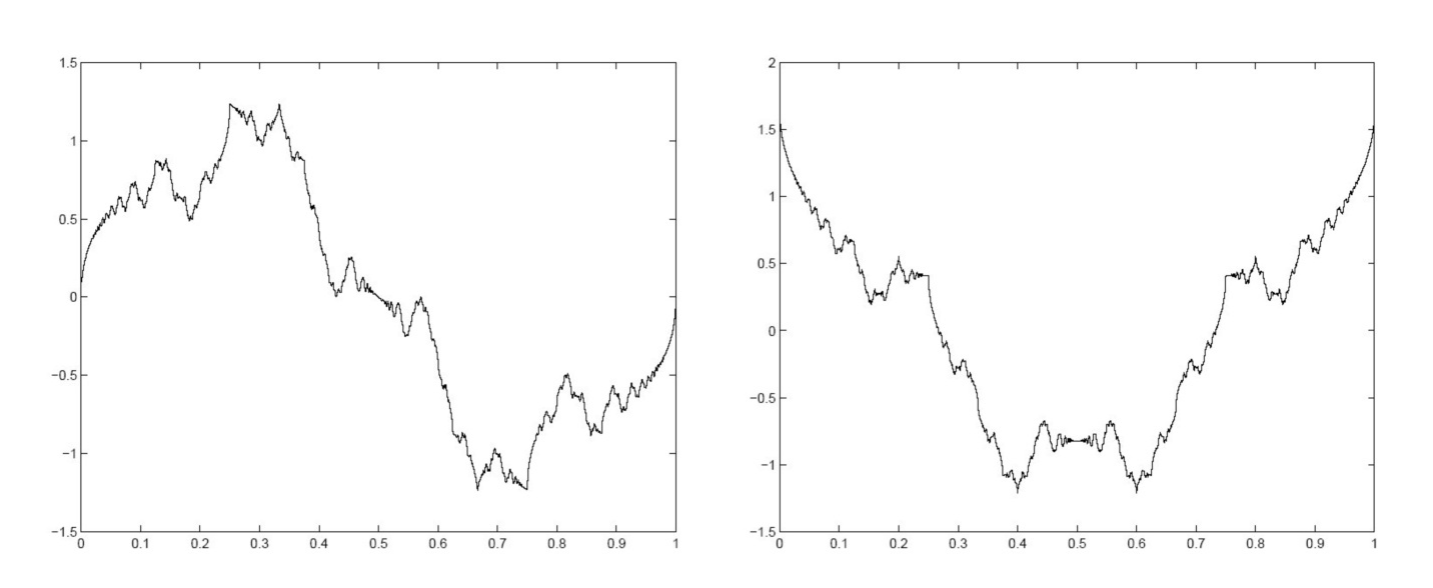
\includegraphics[width=0.7\textwidth]{figs/fig-8-1.png}
\caption{$F_{1}(x)$（左）与 $G_{1}(x)$（右）的图象.}
\label{fig:8.1}
\end{figure}

\begin{figure}[htbp]
\centering
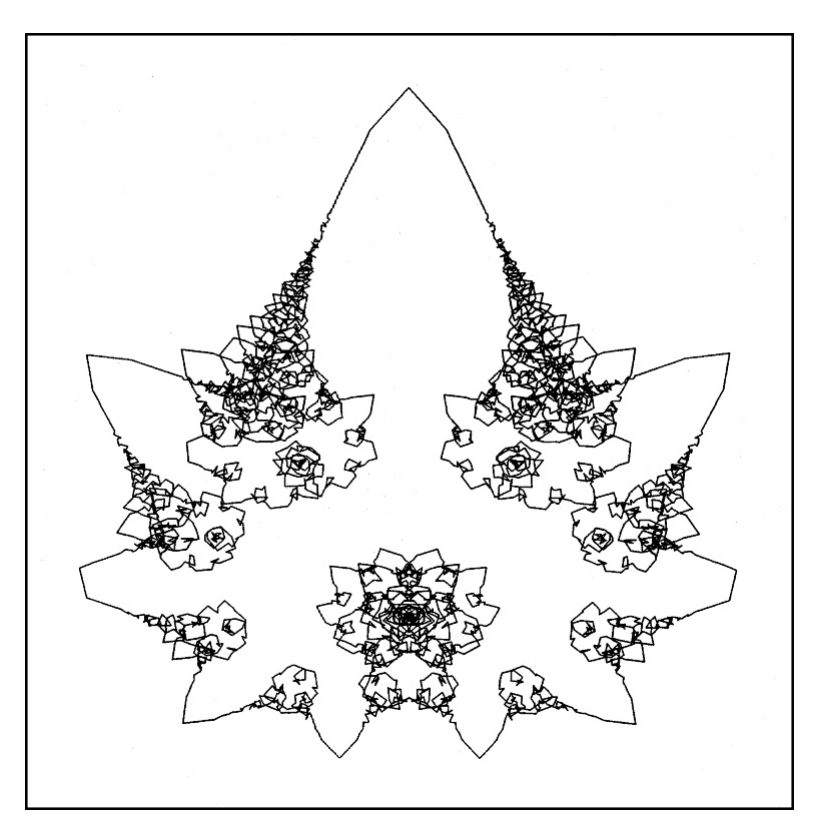
\includegraphics[width=0.42\textwidth]{figs/fig-8-2.png}
\caption{$\sigma(t) = (F_{1/2}(t), G_{1/2}(t))$ 的图象.}
\label{fig:8.2}
\end{figure}

只要 $|x - a/q| \leq 1/q^2$. 对完全和，有显式求值
\begin{align*}
  \sum_{k=1}^{q}e^{2\pi i\frac{a}{q}k^{2}}=\varepsilon_{q}\sqrt{q}\left(\frac{a}{q}\right),\qquad \text{若 } \gcd(a,q)=1,
\end{align*}
其中 $\left(\frac{a}{q}\right)$ 表示 Legendre 符号，而
\begin{align*}
  \varepsilon_{q}=\begin{cases}
    1, & \text{若 } q\equiv 1\pmod 4,\\
    i, & \text{若 } q\equiv 3\pmod 4,\\
    0, & \text{若 } q\equiv 2\pmod 4,\\
    1+i, & \text{若 } q\equiv 0\pmod 4.
  \end{cases}
\end{align*}
给定 $n' = m + q\left[\frac{n-m}{q}\right]$，有
\begin{align*}
  S_{n,m}(a/q)=S_{n'-1,m}(a/q)+S_{n,n'}(a/q)
  =\varepsilon_{q}\left(\frac{a}{q}\right)\frac{n-m}{\sqrt{q}}+O(\sqrt{q}).
\end{align*}
设 $\alpha(a/q; N)$ 是覆盖交集 $\mathrm{graph}(F_\delta) \cap (J_{a/q} \times \R)$ 所需的网格
\begin{align*}
  \mathcal{M}_{N}=\left\{x=\frac{\ell}{N},y=\frac{m}{N};0\leq\ell\leq N\right\}
\end{align*}
的盒子数，设 $\alpha(a/q; N, k)$ 是其中包含于带形 $I_k \times \R$（$I_k = [k/N, (k+1)/N]$）内的盒子数.

(i) 首先证明上界
\begin{align*}
  \overline{\dim}_{\mathrm{B}}(\mathrm{graph}(F_{\delta}))\leq\frac{7}{4}-\frac{\delta}{2}.
\end{align*}
设 $M$ 是待定的正整数. 由 $\alpha(a/q; N, k)$ 的定义，应用均值定理后得
\begin{align*}
  \alpha\Big(\frac{a}{q};N,k\Big)
  &\leq 2+N\sup_{x,y\in I_{k}\cap J_{a/q}}|F_{\delta}(x)-F_{\delta}(y)|\\
  &\leq 2+4\pi\Big|\sum_{n\leq M}n^{1-\delta}e^{2\pi i n^{2}\xi}\Big|
   +N\Big|\sum_{n\geq M}\frac{1}{n^{1+\delta}}\left(e^{2\pi i n^{2}x_{0}}-e^{2\pi i n^{2}y_{0}}\right)\Big|,
\end{align*}
其中 $\xi, x_0, y_0 \in I_k \cap J_{a/q}$. 分部求和给出
\begin{align*}
  \alpha\Big(\frac{a}{q};N,k\Big)
  &\lesssim 4\pi\Big|\sum_{n\leq M}\left[n^{1-\delta}-\left(n+1\right)^{1-\delta}\right]S_{n}(\xi)\Big|\\
  &\quad+\left|S_{M}(\xi)\right|M^{1-\delta}
   +\left(1+\delta\right)N\sum_{n>M}\frac{\left|S_{n,M}(x_{0})\right|+\left|S_{n,M}(y_{0})\right|}{n^{2+\delta}}.
\end{align*}
现在选取 $M = [\sqrt{N}]$，由高斯和的已知估计，得
\begin{align*}
  \alpha\Big(\frac{a}{q};N,k\Big)
  &\lesssim\Big(\frac{M}{\sqrt{q}}+\sqrt{q}\Big)+\Big(\frac{M}{\sqrt{q}}+\sqrt{q}\Big)M^{1-\delta}
   +N\Big[\frac{1}{q^{1/2}}\cdot\frac{1}{N^{\frac{1}{2}(\frac{1}{2}+\delta)}}\Big]\\
  &\lesssim N^{1-\delta/2}\frac{1}{\sqrt{q}}+N^{1/2-\delta/2}\sqrt{q}.
\end{align*}
其次注意
\begin{align*}
  \alpha\Big(\frac{a}{q};N\Big)
  \lesssim\frac{|J_{a/q}|}{1/N}\Big(N^{1-\delta/2}\frac{1}{\sqrt{q}}+N^{1-\delta/2}\sqrt{q}\Big)
  \lesssim\frac{N^{3/2-\delta/2}}{q^{3/2}}+N^{1-\delta/2}\frac{1}{q^{1/2}}.
\end{align*}
于是，覆盖图象所需的网格 $\mathcal{M}_N$ 盒子数以
\begin{align*}
  \sum_{q\leq N^{1/2}}\sum_{(a,q)=1}\left(\frac{N^{3/2-\delta/2}}{q^{3/2}}+N^{1-\delta/2}\frac{1}{q^{1/2}}\right)
  &\lesssim\sum_{q\leq N^{1/2}}\left(\frac{N^{3/2-\delta/2}}{q^{1/2}}+N^{1-\delta/2}q^{1/2}\right)\\
  &\lesssim N^{7/4-\delta/2}
\end{align*}
为界，由此得上界
\begin{align*}
  \overline{\dim}_{\mathrm{B}}(\mathrm{graph}(F_{\delta}))
  \leq\limsup_{N\to\infty}\frac{\log(N^{7/4-\delta/2})}{\log N}
  =\frac{7}{4}-\frac{\delta}{2}.
\end{align*}
显然，同样的证明也表明
\begin{align*}
  \overline{\dim}_{\mathrm{B}}(\operatorname{graph}(G_{\delta}))\leq\frac{7}{4}-\frac{\delta}{2}.
\end{align*}

(ii) 现在证明下界
\begin{align*}
  \underline{\dim}_{\mathrm{B}}(\operatorname{graph}(F_{\delta}))\geq\frac{7}{4}-\frac{\delta}{2},\qquad
  \underline{\dim}_{\mathrm{B}}(\operatorname{graph}(G_{\delta}))\geq\frac{7}{4}-\frac{\delta}{2}.
\end{align*}
这里需要分开两种情形. 对 $F_{\delta}$，选取 $P$ 为满足 $p \equiv 3 \pmod 4$ 且 $p \asymp \sqrt{N}$ 的素数集. 对 $G_{\delta}$，类似进行，但（出于显然的原因）换成素数 $p \equiv 1 \pmod 4$.

由 Minkowski 维数的定义，有
\begin{align*}
  \underline{\dim}_{\mathrm{B}}(\operatorname{graph}(F_{\delta}))
  \geq\liminf_{N\to\infty}\frac{\log\bigl(N\sum_{p\in P}\sum_{0\leq a\leq p}|F_{\delta}(a/p)-F_{\delta}(a/p+1/p^{2})|\bigr)}{\log N}.
\end{align*}
接着，只考虑模 $p$ 的二次剩余所组成的集合 $\mathcal{R}(p)$ 中的 $a$ 值. 这些 $a$ 的相应和大于
\begin{align*}
  \sum_{a\in\mathcal{R}(p)}\Big(F_{\delta}\Big(\frac{a}{p}\Big)-F_{\delta}\Big(\frac{a}{p}+\frac{1}{p^{2}}\Big)\Big)
  &=\operatorname{Im}\Big(\sum_{n}\sum_{r=1}^{(p-1)/2}\frac{e^{2\pi i r^{2}n^{2}/p^{2}}}{n^{1+\delta}}
   \left(1-e^{2\pi i n^{2}/p^{2}}\right)\Big)\\
  &=\operatorname{Im}\Big(\sum_{n}\frac{(-1+i\sqrt{p})\left(1-e^{2\pi i n^{2}/p^{2}}\right)}{2n^{1+\delta}}\Big)\\
  &=\sqrt{p}\sum_{n}\frac{\sin^{2}(\pi n^{2}/p^{2})}{n^{1+\delta}}
   +\sum_{n}\frac{\sin(2\pi n^{2}/p^{2})}{2n^{1+\delta}}
  \gtrsim p^{1/2-\delta}
\end{align*}
的绝对值. 算术级数中的素数定理给出
\begin{align*}
  \underline{\dim}_{\mathrm{B}}(\operatorname{graph}(F_{\delta}))
  \geq\lim_{N\to\infty}\frac{\log\left(N\cdot N^{1/4-\delta/2}\cdot N^{1/2}/\log N^{1/2}\right)}{\log N}
  =\frac{7}{4}-\frac{\delta}{2}.
\end{align*}
\end{proof}

定理 8.11 向高于二次的幂的推广需要数论的若干结果.

解析数论中许多有趣命题的证明，有时可以化归为得到指数和的非平凡上界. 估计这类和的第一种方法由 Weyl 于 1916 年创立，它完全基于下面的引理（见 \cite{b196}）.

\begin{lemma}[Weyl 不等式]\label{lem:8.12}
若 $P$ 是 $k$ 次多项式，$a/q$ 是不可约分数，且多项式 $P$ 的首项系数 $A$ 满足 $|A - a/q| \leq q^{-2}$，则
\begin{align*}
  \sum_{n\leq N}e\left(P(n)\right)
  \lesssim\left(N q^{-1/K}+N^{1-1/K}+N^{1-k/K}q^{1/K}\right)N^{\varepsilon}
\end{align*}
对 $K = 2^{k-1}$ 与每个 $\varepsilon > 0$ 成立.
\end{lemma}

用归功于 I.~M.~Vinogradov 的方法，可以对大的 $k$ 改进 Weyl 不等式. Vinogradov 方法可以得到若干类结果，下面这个取自 \cite{b184} 的 Th\'eor\`eme 10.1（对陈述略作简化）.

\begin{lemma}\label{lem:8.13}
设 $P, k, A$ 与 $q$ 如 Weyl 不等式. 则对 $k \geq 9$ 与 $N \leq q \leq N^{k-2}$，有估计
\begin{align*}
  \sum_{n\leq N}e(P(n))\lesssim N^{1-\delta},
\end{align*}
其中 $\delta = (9k^2\log k)^{-1}$.
\end{lemma}

在某些语境中（例如研究素数之和时），指数和出现时带有只能被平均地控制的系数，因而分部求和不适用. 大筛不等式允许在某些情形下，若这类指数和的个数足够多，则获得相消. 大筛不等式依语境有若干表述；也许最简单的如下（见 \cite{b172}）.

\begin{lemma}[大筛不等式]\label{lem:8.14}
设 $\delta > 0$，$\{t_\nu\}_{\nu=1}^R$ 满足 $0 \leq t_1 < t_2 < \cdots < t_R < 1 - \delta$，且 $t_{\nu+1} - t_\nu > \delta$. 则
\begin{align*}
  \sum_{\nu=1}^{R}\Big|\sum_{n\leq N}a_{n} e\left(n t_{\nu}\right)\Big|^{2}
  \leq\left(N+\delta^{-1}\right)\sum_{n\leq N}|a_{n}|^{2}
\end{align*}
对任意复数 $a_{n}$ 成立.
\end{lemma}

现在考虑函数族
\begin{align*}
  F_{\alpha,k}(x)=\sum_{n=1}^{\infty}\frac{c_{n} e(n^{k} x)}{n^{\alpha}},\qquad
  0<\varliminf c_{n}\leq\varlimsup c_{n}<\infty.
\end{align*}
可以计算它们图象的分形维数.

\begin{theorem}\label{thm:8.15}
若 $(k+1)/2 \leq \alpha \leq k+1/2$，则
\begin{align*}
  \dim(F_{\alpha,k})=2+\frac{1}{2k}-\frac{\alpha}{k}.
\end{align*}
\end{theorem}

\begin{remark}\label{rem:8.16}
注意这一结果蕴含: 对 $(k+1)/2 \leq \alpha < k+1/2$，$F_{\alpha,k}$ 的分形维数是非整数. 另一方面，若 $\alpha > k+1/2$，则 $F_{\alpha,k}$ 绝对连续（注意 $F_{\alpha,k}' \in L^2$），分形维数平凡地等于一. 在猜想界 $\|\sum_{n \leq N} c_n e(n^k x)\|_{2k} = O(N^{1/2+\varepsilon})$（对 $k = 2$ 成立）之下，范围可以补全到 $1 < \alpha \leq k+1/2$.
\end{remark}

\begin{proof}[定理~\ref{thm:8.15} 的证明]
首先证明上界
\begin{equation}\label{eq:8.3}
  \overline{\dim}(F_{\alpha,k})\leq 2+\frac{1}{2k}-\frac{\alpha}{k}.
\end{equation}
给定 $x, y \in I$，其中 $I$ 是长度为 $h$ 的闭区间，把 $F_{\alpha, k}$ 的项按 $n > h^{-1/(k-1)}$ 分开，并对 $n \leq h^{-1/k}$ 的项应用均值定理. 则得到
\begin{align*}
  |F_{\alpha,k}(x)-F_{\alpha,k}(y)|
  \lesssim h\left|S_{1}(\xi)\right|+|S_{2}(x)|+|S_{2}(y)|+h^{(\alpha-1)/(k-1)},
\end{align*}
其中
\begin{align*}
  S_{1}(\xi)=\sum_{n\leq h^{-1/k}}c_{n}n^{k-\alpha}e(n^{k}\xi),\qquad
  S_{2}(t)=\sum_{h^{-1/k}<n\leq h^{-1/(k-1)}}\frac{c_{n}e(n^{k}t)}{n^{\alpha}},
\end{align*}
$\xi \in I$. 取 $I = I_j$（$I_j$ 如分形维数定义中），并分离 $j$ 为奇、偶时对 $A_h$（定义于注 8.10）的贡献，有
\begin{equation}\label{eq:8.4}
  A_{h}\lesssim\sum_{\nu}\left|S_{1}(t_{\nu})\right|
  +h^{-1}\sum_{\nu}\left|S_{2}(t_{\nu}^{\prime})\right|
  +h^{(\alpha-2k+1)/(k-1)},
\end{equation}
其中 $h < t_{\nu+1} - t_{\nu}$，$t_{\nu+1}^{\prime} - t_{\nu}^{\prime} < 3h$.

把 $S_{2}$ 细分成二进区间，得
\begin{align*}
  S_{2}(t_{\nu}^{\prime})\lesssim\sum_{M}\Big|\sum_{M<n\leq 2M}\frac{c_{n}e(n^{k}t_{\nu}^{\prime})}{n^{\alpha}}\Big|,
\end{align*}
其中 $M = 2^m h^{-1/k}$，$h^{-1/k} \leq M < h^{-1/(k-1)}$. 再把每个二进区间 $(M, 2M]$ 细分为长度 $h^{-1}M^{1-k}$ 的区间，对每个 $M$ 找到 $M_1$ 与 $M_2$，使 $M < M_1 < M_2 \leq 2M$，$M_2 < M_1 + h^{-1}M^{1-k}$，且
\begin{align*}
  \sum_{\nu}|S_{2}(t_{\nu}^{\prime})|
  \lesssim\sum_{M}\frac{M}{h^{-1}M^{1-k}}\sum_{\nu}
  \Big|\sum_{M_{1}<n\leq M_{2}}\frac{c_{n}e(n^{k}t_{\nu}^{\prime})}{n^{\alpha}}\Big|.
\end{align*}
记最内层的和为 $S_{2M}(t'_\nu)$. 则由 \eqref{eq:8.4} 与 Cauchy 不等式，得
\begin{equation}\label{eq:8.5}
  A_{h}^{2}\lesssim h^{-1}\sum_{\nu}|S_{1}(t_{\nu})|^{2}
  +h^{-1}\sum_{M}M^{2k+\varepsilon}\sum_{\nu}|S_{2M}(t_{\nu}^{\prime})|^{2}
  +h^{(2\alpha-4k+2)/(k-1)}.
\end{equation}
大筛不等式蕴含
\begin{align*}
  \sum_{\nu}|S_{1}(t_{\nu})|^{2}
  \lesssim(h^{-1}+h^{-1})\sum_{n\leq h^{-1/k}}|c_{n}|^{2}n^{2k-2\alpha}
  \lesssim h^{-3+(2\alpha-1)/k-\varepsilon},
\end{align*}
以及
\begin{align*}
  \sum_{\nu}|S_{2M}(t_{\nu}^{\prime})|^{2}
  \lesssim(h^{-1}+h^{-1})\sum_{M_{1}<n<M_{2}}|c_{n}|^{2}M^{-2\alpha}
  \lesssim h^{-2}M^{1-k-2\alpha}.
\end{align*}
因此，代入 \eqref{eq:8.5},
\begin{align*}
  A_{h}^{2}\lesssim h^{-4+(2\alpha-1)/k-\varepsilon},
\end{align*}
由此得 \eqref{eq:8.3}.

现在证明下界
\begin{equation}\label{eq:8.6}
  \underline{\dim}(F_{\alpha,k})\geq 2+\frac{1}{2k}-\frac{\alpha}{k}.
\end{equation}
设
\begin{align*}
  f(x)=F_{\alpha,k}(x+h)-F_{\alpha,k}(x).
\end{align*}
由 $A_{h}$ 的定义与 Hölder 不等式,
\begin{equation}\label{eq:8.7}
  A_{h}\geq h^{-2}\|f\|_{1}\geq h^{-2}\frac{\|f\|_{2}^{3}}{\|f\|_{4}^{2}}.
\end{equation}
Parseval 恒等式证明
\begin{align*}
  \|f\|_{2}^{2}=\sum_{n}|c_{n}|^{2}\frac{|1-e(n^{k}h)|^{2}}{n^{2\alpha}}.
\end{align*}
只考虑 $1/(4h) < n^{k} < 3/(4h)$ 的贡献，得到
\begin{align*}
  \|f\|_{2}^{2}\gtrsim h^{(2\alpha-1)/k}.
\end{align*}
另一方面，细分成二进区间后，对每个 $\varepsilon > 0$ 有
\begin{align*}
  \|f\|_{4}^{4}\lesssim\sup_{N}N^{\varepsilon}
  \Big\|\sum_{N\leq n<2N}c_{n}\frac{1-e(n^{k}h)}{n^{\alpha}}e(n^{k}x)\Big\|_{4}^{4},
\end{align*}
从而再次用 Parseval 恒等式,
\begin{align*}
  \|f\|_{4}^{4}\lesssim\sup_{N}N^{\varepsilon-4\alpha}
  \sum_{N\leq n<2N}\sum_{N\leq m<2N}
  |r_{k}\left(n^{k}+m^{k}\right)|^{2}|c_{n}|^{2}|c_{m}|^{2}
  |1-e(n^{k}h)|^{2}|1-e(m^{k}h)|^{2},
\end{align*}
其中 $r_k$ 表示表为两个 $k$ 次幂之和的表法个数. 有 $r_k(l) \lesssim l^{\varepsilon}$（因为 $l = m^k + n^k$ 蕴含: 若 $k$ 为奇，$m + n$ 整除 $l$；若 $k$ 为偶，$m^{k/2} + in^{k/2}$ 在 $\Z[i]$ 中整除 $l$；而因子个数增长得比任何正幂都慢）. 则
\begin{align*}
  \|f\|_{4}^{4}
  &\lesssim\sup_{N}N^{\varepsilon-4\alpha}
   \Big(\sum_{N\leq n<2N}|c_{n}|^{2}|1-e(n^{k}h)|^{2}\Big)^{2}\\
  &\lesssim\sup_{N}N^{\varepsilon-4\alpha}\min\left(N^{2},N^{2+2k}h^{-2}\right)
  \lesssim h^{(4\alpha-2)/k-\varepsilon}.
\end{align*}
把 $\|f\|_2$ 与 $\|f\|_4$ 的界代入 \eqref{eq:8.7}，得出
\begin{align*}
  A_{h}\gtrsim h^{-2-1/2k+\alpha/k+\varepsilon}
\end{align*}
对每个 $\varepsilon > 0$ 成立，这蕴含 \eqref{eq:8.6}.
\end{proof}

\section{晶体学部分和的收敛与发散}

取函数 $f \in L^{1}(\T)$，考虑其傅里叶级数
\begin{align*}
  \sum_{k=-\infty}^{\infty}\widehat{f}(k)e^{2\pi i k x},
\end{align*}
其中 $\widehat{f}(k)=\int_{0}^{1}f(x)e^{-2\pi i k x}\,\mathrm{d}x$. 这里 $\T$ 以通常方式等同于 $[0, 1)$. 通过傅里叶系数 $(\widehat{f}(k))_{k \in \Z}$ 重建函数 $f$ 的传统方式是考虑 $N$-部分和
\begin{equation}\label{eq:8.8}
  S_{N}f(x)=\sum_{|k|\leq N}\widehat{f}(k)\,e^{2\pi i k x}.
\end{equation}
众所周知有范数收敛: 若 $f \in L^p(\T)$，$1 < p < \infty$，则当 $N\to\infty$ 时
\begin{align*}
  S_{N}f\to f\quad\text{于 } L^{p}(\T).
\end{align*}
而自 Carleson \cite{b175}（其后 Hunt \cite{b191}）以来，还知道有几乎处处收敛.

然而，考虑到把傅里叶系数解释为周期分布的衍射图样，似乎更自然的做法是关注那些给我们更多信息的系数，即模更大的系数，并按傅里叶系数的模递减顺序重建函数. 即，对每个 $\lambda > 0$ 考虑部分和
\begin{equation}\label{eq:8.9}
  \tilde{S}_{\lambda}f(x)=\sum_{|\widehat{f}(k)|>\lambda}\widehat{f}(k)e^{2\pi i k x},
\end{equation}
以及它们在 $\lambda \to 0$ 时的极限.

1996 年，见 \cite{b192}，T.~W.~Körner 否定了 L.~Carleson 与 R.~Coifman 提出的一个问题，证明了存在函数 $f \in L^2(\T)$，使
\begin{equation}\label{eq:10}
  \limsup_{\lambda\to 0^{+}}\Big|\sum_{|\widehat{f}(k)|\geq\lambda}\widehat{f}(k)e^{2\pi i k x}\Big|=\infty
  \quad\text{对几乎每个 } x\in\T.
\end{equation}
当按递减系数求和时傅里叶级数的这种``坏''行为，例如与其他基（如小波）的情形形成对照，见 \cite{b195}.

Körner 的证明基于对归功于 Olevskii 的构造的巧妙修改，还用到 R.~Salem 与 A.~Zygmund 的一个概率引理. 具有所需性质的函数没有显式构造.

\section*{一个用高斯和的构造}

利用高斯和，可以产生满足 \eqref{eq:10} 的函数 $f \in L^p(\T)$（$p < 4/3$）的显式例子. 注意这个 $p$ 的范围，并与 Körner 的结果比较.

构造如下. 固定 $\varepsilon > 0$. 对每个 $k \geq 0$，取
\begin{equation}\label{eq:11}
  f_{k}(x)=\sum_{n=2^{2k}}^{2^{2k+2}-1}a_{n}\cos(2\pi n x),
\end{equation}
其中
\begin{align*}
  a_{n}=\begin{cases}
    \frac{1}{2^{k/2-k\varepsilon}}\left(1+\frac{1}{n}\right), & \text{若 } n \text{ 是完全平方数},\\
    \frac{1}{2^{k/2-k\varepsilon}}\left(1-\frac{1}{2^{2k}}\right), & \text{其他},
  \end{cases}
\end{align*}
并令
\begin{equation}\label{eq:12}
  f(x)=1+2\sum_{k=1}^{\infty}f_{k}(x).
\end{equation}
可以验证
\begin{align*}
  \|f_{k}\|_{p}\simeq 2^{k(\varepsilon+3/2-2/p)},
\end{align*}
因此，取足够小的 $\varepsilon$，函数 $f$（定义于 \eqref{eq:12}）对每个 $p < 4/3$ 都属于 $L^p(\T)$.

$f(x)$ 的系数（频谱）在对应 $f_{k}(x)$ 与 $f_{k+1}(x)$ 的两个相邻块上的外观如下所示.

\begin{center}
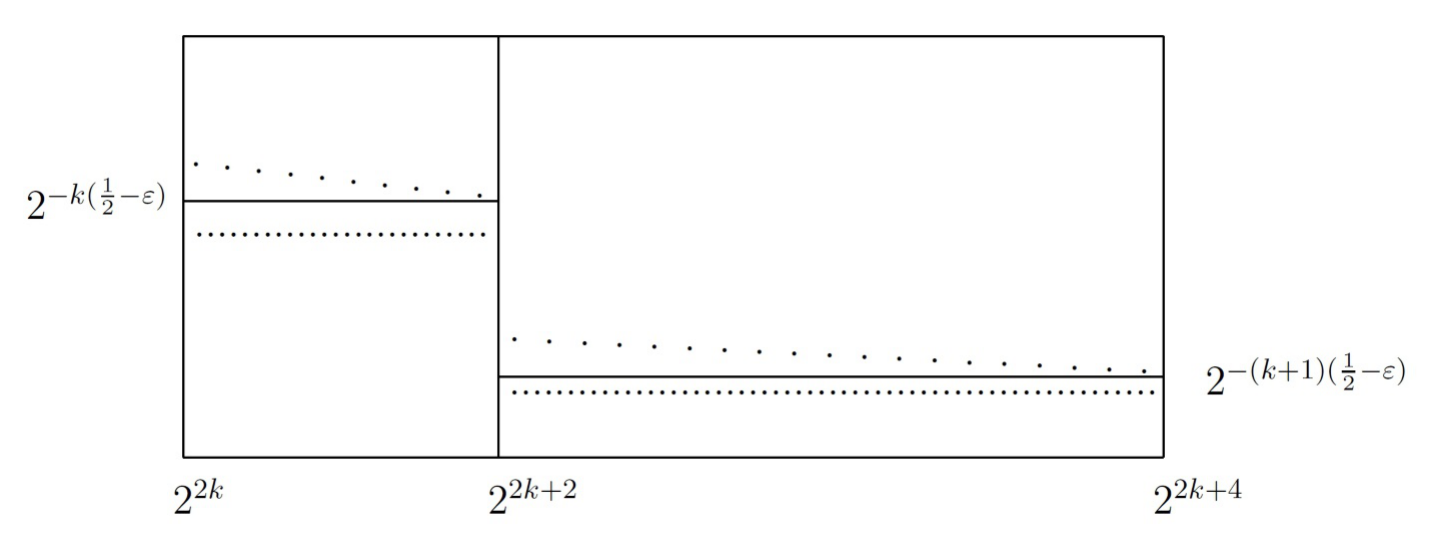
\includegraphics[width=0.78\textwidth]{figs/fig-8-sigma.png}
\end{center}

注意，对
\begin{equation}\label{eq:13}
  b_{k}=\frac{1}{2^{k\left(1/2-\varepsilon\right)}}\left(1+\frac{1}{j}\right),
\end{equation}
其中 $j = j(k)$ 满足 $2^{2k} \leq j < 2^{2k+2}$，由上面函数 $f$ 的定义，有
\begin{align*}
  \sum_{|\widehat{f}(\nu)|>b_{k}}\widehat{f}(\nu)e^{2\pi i\nu x}
  &=\sum_{|\nu|\leq 2^{2k}}\widehat{f}(\nu)e^{2\pi i\nu x}
   +\frac{1}{2^{k(1/2-\varepsilon)}}\sum_{2^{2k}\leq m^{2}<2^{2k}+j}
   \left(1+\frac{1}{m^{2}}\right)e^{2\pi i m^{2}x}.
\end{align*}
于是，当 $k \to \infty$ 时，回忆 Carleson--Hunt 收敛结果，对几乎所有 $x \in \R$,
\begin{equation}\label{eq:14}
  \Big|\sum_{|\widehat{f}(\nu)|>b_{k}}\widehat{f}(\nu)e^{2\pi i\nu x}\Big|
  =\frac{1}{2^{k(1/2-\varepsilon)}}\Big|\sum_{2^{2k}\leq m^{2}<2^{2k}+j}e^{2\pi i m^{2}x}\Big|
  +O(1).
\end{equation}
现在回忆下面的事实.

\begin{fact}\label{fact:8.17}
若 $|x - y| \leq 1/M^2$，则
\begin{align*}
  \sup_{1\leq k\leq M}\Big|\sum_{j=M}^{M+k}e^{2\pi i j^{2}x}\Big|
  \geq C\sup_{1\leq k\leq M}\Big|\sum_{j=M}^{M+k}e^{2\pi i j^{2}y}\Big|.
\end{align*}
\end{fact}

\begin{fact}\label{fact:8.18}
若 $\gcd(P, Q) = 1$，$M/2 \leq Q \leq M$ 且 $Q$ 为奇数，则
\begin{align*}
  \sup_{1\leq k\leq M}\Big|\sum_{j=M}^{M+k}e^{2\pi i j^{2}P/Q}\Big|\geq\sqrt{Q}.
\end{align*}
\end{fact}

事实 8.17 由分部求和得出，而事实 8.18 是定理 7.6 的推论.

我们将按 $x$ 构造 \eqref{eq:13} 中的序列 $b_k$. 设 $x \in [0,1]$ 是无理数，考虑其连分数展开的渐近分数序列 $\{P_m/Q_m\}$. 它们满足 $\gcd(P_m, Q_m) = 1$ 与
\begin{align*}
  \left|\frac{P_{m}}{Q_{m}}-x\right|<\frac{1}{Q_{m}^{2}}.
\end{align*}
奇数分母 $Q_{n}$ 有无穷多个.

奇数分母的（子）序列 $\{Q_{\alpha}\}$ 确定二进块
\begin{equation}\label{eq:15}
  2^{k_{\alpha}}\leq Q_{\alpha}\leq 2^{k_{\alpha}+1}.
\end{equation}
用这个指标序列 $\{k = k_\alpha\}$，考虑 \eqref{eq:13} 中的数 $b_k$，其中 $j = j(k)$ 选取为使
\begin{align*}
  \Big|\sum_{2^{2k}\leq m^{2}<2^{2k}+j}e^{2\pi i m^{2}x}\Big|
  =\sup_{1\leq\ell\leq 2^{k}}\Big|\sum_{s=2^{k}}^{2^{k}+\ell}e^{2\pi i s^{2}x}\Big|.
\end{align*}
先用事实 8.17，再用事实 8.18，得
\begin{align*}
  \sup_{1\leq\ell\leq 2^{k}}\Big|\sum_{s=2^{k}}^{2^{k}+\ell}e^{2\pi i s^{2}x}\Big|
  \geq C\sup_{1\leq\ell\leq 2^{k}}\Big|\sum_{s=2^{k}}^{2^{k}+\ell}e^{2\pi i s^{2}P_{\alpha}/Q_{\alpha}}\Big|
  \geq C\sqrt{Q_{\alpha}}.
\end{align*}
最后，由 \eqref{eq:14} 与 \eqref{eq:15}，得出
\begin{align*}
  \Big|\sum_{|\widehat{f}(\nu)|>b_{k}}\widehat{f}(\nu)e^{2\pi i\nu x}\Big|
  \geq C2^{k\varepsilon}+O(1).
\end{align*}
这证明函数 $f$ 满足 \eqref{eq:10} 中的几乎处处发散性质.

\subsection{范数中的收敛/发散}

还可以证明 $L^p$-收敛（$p < 2$）对 \eqref{eq:8.9} 的部分和 $\tilde{S}_\lambda$ 也失败. 更具体地，有下面.

\begin{theorem}\label{thm:8.19}
对所有 $p$，$1 \leq p < 2$，存在（显式构造的）函数 $f \in L^p(\T)$，使
\begin{align*}
  \limsup_{\lambda\to 0^{+}}\|\tilde{S}_{\lambda}f\|_{p}=\infty.
\end{align*}
\end{theorem}

这个函数的构造也是数论性质的，与上面展示的构造类似，但以素数指标扮演完全平方数的角色. 细节见 \cite{b182}.

可以论证，$\tilde{S}_{\lambda}f$ 收敛失败的一个原因是测不准原理未被考虑: 对 $|\widehat{f}(k)|$ 的大小施加限制而不对 $|k|$ 本身施加限制是没有意义的. 给定递减函数 $\phi$，可以考虑部分和:
\begin{align*}
  S_{N}^{\phi}f(x)=\sum_{\substack{|k|\leq N\\ |\widehat{f}(k)|\geq\phi(N)}}\widehat{f}(k)e^{2\pi i k x}.
\end{align*}
于是我们的构造表明，$S_{N}^{\phi}$ 在范数中收敛或发散的不同行为取决于条件
\begin{align*}
  N\cdot\phi^{2}(N)=o(1).
\end{align*}
特别地，对 $\phi(N) = N^{-\delta}$，$\delta > 0$，$S_{N}^{\delta}f$ 在 $L^{p}$-范数（$p < 2$）中的收敛
\begin{align*}
  S_{N}^{\delta}f(x)=\sum_{\substack{|k|\leq N\\ |\widehat{f}(k)|\geq N^{-\delta}}}\widehat{f}(k)e^{2\pi i k x}
\end{align*}
要求指数 $\delta > 1/2$，这与测不准原理相当吻合. 见 \cite{b182}.

% ================================================================
% 编号审计 (第 8 章):
%   question   ques:8.1  → 问题 8.1   (§8.1)
%   question   ques:8.2  → 问题 8.2   (§8.1)
%   definition def:8.3   → 定义 8.3   (§8.2，B_2[∞]-序列)
%   theorem    thm:8.4   → 定理 8.4   (§8.2)
%   lemma      lem:8.5   → 引理 8.5   (§8.2)
%   remark     rem:8.6   → 注 8.6     (§8.2)
%   proposition prop:8.7  → 命题 8.7   (§8.3)
%   lemma      lem:8.8   → 引理 8.8   (§8.3)
%   lemma      lem:8.9   → 引理 8.9   (§8.3)
%   remark     rem:8.10  → 注 8.10    (§8.4)
%   theorem    thm:8.11  → 定理 8.11  (§8.4，[176])
%   lemma      lem:8.12  → 引理 8.12 (Weyl 不等式) (§8.4)
%   lemma      lem:8.13  → 引理 8.13 (Vinogradov) (§8.4)
%   lemma      lem:8.14  → 引理 8.14 (大筛不等式) (§8.4)
%   theorem    thm:8.15  → 定理 8.15  (§8.4)
%   remark     rem:8.16  → 注 8.16    (§8.4)
%   fact       fact:8.17 → 事实 8.17 (§8.5)
%   fact       fact:8.18 → 事实 8.18 (§8.5)
%   theorem    thm:8.19  → 定理 8.19  (§8.5)
%   公式: eq:8.1 (§8.2 下界)，eq:8.2 (§8.2 断言)，eq:8.3 (§8.4 上界),
%         eq:8.4 (§8.4 A_h 界)，eq:8.5 (§8.4 A_h²)，eq:8.6 (§8.4 下界),
%         eq:8.7 (§8.4 Hölder 不等式)，eq:8.8 (§8.5 N-部分和),
%         eq:8.9 (§8.5 λ-部分和)，eq:8.10 (§8.5 发散性质),
%         eq:8.11 (§8.5 f_k)，eq:8.12 (§8.5 f)，eq:8.13 (§8.5 b_k),
%         eq:8.14 (§8.5 主项)，eq:8.15 (§8.5 二进块)
%   注: eq:8.10/8.11/8.12/8.13/8.14/8.15 的标签在原书中即 (8.10)-(8.15)；
%       本节无编号小标题"一个用高斯和的构造"用 \section*{}.
%   \cite 使用: b24 b171 b172 b173 b174 b175 b176 b180 b182 b184 b185
%               b187 b188 b189 b191 b192 b194 b195 b196
% ================================================================
